% slides.tex

% A demo of the Prosper documentclass for \LaTeX
%
% The layout and colors in this demo are designed to look best with
% UMBC's Prosper styles.  The demo should compile with any other Prosper
% style, however the results will not be ideal because slide dimensions,
% fonts sizes and color pallets vary widely from style to style.
% 
% When you create your own Prosper document, first you pick a style,
% then lay out the contents to fit that specific style.
% 
% You may want to have a look at the tutorial in:
%     http://www.math.umbc.edu/~rouben/prosper/
% 
% Rouben Rostamian <rostamian@umbc.edu>
% January 2003

\documentclass[pdf,umbc4,slideColor,colorBG]{prosper}
\ptsize{9}

\title{Fluid Flow Through a Porous Medium}
\subtitle{A demo of the Prosper documentclass for \LaTeX}
\author{Rouben Rostamian}
\email{rostamian@umbc.edu}
\institution{
	Department of Mathematics and Statistics \\
	University of Maryland Baltimore County \\
	Baltimore, MD 21250, USA
}

% The following block of lines are specific to this document.
% DONT'T COPY THEM TO YOUR documents if you don't need them.
\newcommand{\pd}[2]{\frac{\partial #1}{\partial #2}}	% partial derivatives
\renewcommand{\div}{\mathop\mathrm{div}\nolimits}	% divergence
\newcommand{\header}[1]{\textbf{\textsl{{\blue #1}}}}	% a convenience macro
\newcommand{\highlight}[1]{% highlight text as with a yellow marker
	\psframebox[fillstyle=solid,fillcolor=yellow,linestyle=none]{#1}%
}

% set up hyperlink colors
\hypersetup{colorlinks=true,anchorcolor=green,linkcolor=red,menucolor=cyan}

% If using a umbc* style, we add a logo and navigation icons 
% The navigation icons look like this:   " <--   O  -->"
% In the Acrobat Reader, if you click on an icon by the left mouse button:
%   o the left icon takes you to the first slide
%     (it's equivalent to Control-Shift-PageUp)
%   o the right icon takes you to the last slide
%     (it's equivalent to Control-Shift-PageDown)
%   o the middle icon takes you to the last viewed slide.  Use it to
%     return to the previous page after a hyperlink jump.
%     (it's equivalent to Control-LeftArrow)
%
% REMOVE THE FOLLOWING BLOCK OF LINES entirely if you don't care for the UMBC
% logo and navigation icons.
\usepackage{ifthen}
\ifthenelse{\not\isundefined{\umbclogo}}{%
\usepackage{amssymb}%
\Logo{%
	\umbclogo
	\hspace{5cm}
	\tiny
	\Acrobatmenu{FirstPage}{$\rule{0.20ex}{1ex}\!\!\blacktriangleleft$}
	\qquad
	\Acrobatmenu{GoBack}{$\circlearrowright$}
	\qquad
	\Acrobatmenu{LastPage}{$\blacktriangleright\!\!\rule{0.20ex}{1ex}$}
}}{}

% The "pst-node" package is used in the slide titled:
%           "Boundary conditions derived from symmetries".
% Most users won't need this.
% DON'T COPY THIS TO YOUR documents unless you know what it does.
\usepackage{pst-node}

\begin{document}

%-------------------------------------------------------------------- Slide --

\maketitle

%-------------------------------------------------------------------- Slide --

\overlays{2}{
\begin{slide}{Overview}

\bigskip

\begin{itemize}

\item
	Fluid flow through a lattice of solid objects
\item
	Homogenization via a formal asymptotic expansion
\item
	Reduction to Darcy's Law -- the permeability tensor
\item
	Symmetries of the unit-cell problem
\item
	Formulation of the unit cell problem \textit{a la} Femlab
\item
	Sample solutions obtained by Femlab
\item
	Plans for future work

\end{itemize}

\bigskip

\fromSlide{2}{
\footnotesize
\textsl{Reference}:

\smallskip

Enrique S{\'a}nchez-Palencia.
{\em Nonhomogeneous media and vibration theory}, volume 127 of {\em
Lecture Notes in Physics}.  Springer-Verlag, Berlin, 1980.
} % end of fromSlide

\end{slide}
}
%-------------------------------------------------------------------- Slide --

\overlays{2}{
\begin{slide}{The Navier-Stokes equations}
\hypertarget{Stokes}{}

\bigskip

The Navier-Stokes equations:

\[
\begin{array}{l}
\displaystyle
	\rho \, ( \pd{v}{t} + (\nabla v) v ) = \mu\Delta v - \nabla p +  f \\
	\div v = 0
\end{array}
\]

\textcolor{magenta}{Given:}
	$\rho$: density, $\mu$ = viscosity, $ f$ = force per unit volume, 
\newline
\textcolor{magenta}{Unknowns:}
	$ v$ = the velocity field, $p$ = the pressure field

\bigskip

\fromSlide{2}{
The Stokes equations:
\newgray{lightgray}{0.8}

\[
\begin{array}{l}
\displaystyle
	\rho \pd{ v}{t} {\lightgray + \rho (\nabla v) v}
		= \mu\Delta v - \nabla p +  f \\
	\div v = 0
\end{array}
\]

{\scriptsize Good when dynamic (inertia) forces are ``small'' compared
to viscous forces}

} % fromSlide
\end{slide}
}

%-------------------------------------------------------------------- Slide --

\begin{slide}{Systems of equations}

\[
\begin{array}{ll}

\hypertarget{P0}{(P_0)} &

\left\{
\begin{array}{l}
\Delta_y  v^{0} = 0 \\
\div_y  v^{0} = 0
\end{array}
\right.

\bigskip \\

\hypertarget{P1}{(P_1)} &

\left\{
\begin{array}{l}
	\Delta_y  v^{1} + \nabla_y \div_x  v^{0} + \nabla_x \div_y  v^{0}
		- \nabla_y p^{0} = 0 \\
	\div_y  v^{1}  + \div_x  v^{0} = 0
\end{array}
\right.

\bigskip \\

\hypertarget{P2}{(P_2)} &

\left\{
\begin{array}{l}
	\Delta_y  v^{2} + \nabla_y \div_x  v^{1}
		+ \nabla_x \div_y  v^{1} + \Delta_x  v^{0} - \nabla_y p^{1}
		- \nabla_x p^{0} + f = 0 \\
	\div_y  v^{2}  + \div_x  v^{1} = 0
\end{array}
\right.

\bigskip \\

\hypertarget{P3}{(P_3)} &

\left\{
\begin{array}{l}
	\Delta_y  v^{3} + \nabla_y \div_x  v^{2}
		+ \nabla_x \div_y  v^{2} \mbox{} + \Delta_x  v^{1}
		- \nabla_y p^{2} - \nabla_x p^{1} = 0 \\
	\div_y  v^{3}  + \div_x  v^{2} = 0
\end{array}
\right.

\end{array}
\]

\end{slide}

%-------------------------------------------------------------------- Slide --

\overlays{2}{
\begin{slide}{Analysis}

\header{Look at \hyperlink{P0}{$(P_0)$}:}
\[
	\left\{
	\begin{array}{l}
		\Delta_y  v^{0} = 0 \\
		\div_y  v^{0} = 0
	\end{array}
	\right.
\]
\[
	\Rightarrow
	\quad
	\int_{\partial Y}  v^{0} \cdot (\nabla  v^{0})  n \, da
		- \int_Y | \nabla  v^{0} |^2 \, dy = 0
	\quad
	\Rightarrow
	\quad
	\highlight{ v^{0}(x,y) \equiv 0}
\]

\bigskip

\fromSlide{2}{
\header{Look at reduced \hyperlink{P1}{$(P_1)$}:}
\[
	\left\{
	\begin{array}{l}
		\Delta_y  v^{1} - \nabla_y p^{0} = 0 \\
		\div_y  v^{1}= 0
	\end{array}
	\right.
\]
\[
	\Rightarrow
	\quad
	\int_{\partial Y}  v^{1} \cdot \bigl[(\nabla_y  v^{1})  n \bigr] \, da
		- \int_Y | \nabla_y  v^{1} |^2 \, dy
		- \int_{\partial Y} p^{0} \,  v^{1} \cdot  n \, da
		+ \int_Y p^{0} \div_y  v^{1} \, dy = 0
\]
\[
	\Rightarrow
	\quad
	\highlight{ v^{1}(x,y) \equiv 0}
	\Rightarrow
	\quad
	\highlight{p^{0} = p^{0}(x)}
\]
} % end of fromSlide

\end{slide}
} % end overlays

%-------------------------------------------------------------------- Slide --

\overlays{4}{
\begin{slide}{Analysis continued}

\header{Look at reduced \hyperlink{P2}{$(P_2)$}:}
\[
\left\{
	\begin{array}{l}
		\Delta_y  v^{2}(x,y) - \nabla_y p^{1}(x,y)
			- \nabla_x p^{0}(x) +  f(x) = 0 \\
		\div_y  v^{2}(x,y) = 0
	\end{array}
	\right.
\]

\fromSlide{2}{
\header{Function space:}
\[
	\highlight{
		V_Y = \left\{  w \in [H^1_\mathrm{per}(Y)]^n : 
		\div  w = 0, \left. w\right|_{\Gamma_s}  = 0 \right\}
	}
\]
} % end of fromSlide

\fromSlide{3}{
\header{Arbitrary test-function $ w \in V_Y$:}
\[
\begin{array}{ll}
\lefteqn{\int_{\partial Y} \bigl[(\nabla_y  v^{2})  n \bigr] \cdot  w \, da
	- \int_Y \nabla_y  v^{2} \cdot \nabla  w \, dy} \qquad
	\\
	& \displaystyle \mbox{}
	- \int_{\partial Y} p^{1} \,  w \cdot  n \, da
	+ \int_Y p^{1} \div_y  w \, dy
	+ \bigl(- \nabla_x p^{0}(x) +  f(x)\bigr) \cdot \int_Y  w \, dy = 0.
\end{array}
\]
} % end of fromSlide

\fromSlide{4}{
\header{Variational problem:}
\[
	\int_Y \nabla_y  v^{2} \cdot \nabla  w \, dy = 
		\bigl( f(x) - \nabla_x p^{0}(x)\bigr) \cdot \int_Y  w \, dy
\]
} % end of fromSlide

\end{slide}
} % end overlays

%-------------------------------------------------------------------- Slide --

\overlays{4}{
\begin{slide}{Convergence to homogenized solution}
\hyperlink{Stokes}{{Recall}} the steady-state Stokes' equations with $\mu=1$:
\[
	\begin{array}{l}
		\Delta v^\epsilon - \nabla p^\epsilon +  f  = 0
			\quad \mbox{in }\Omega_\epsilon \\
		\div v^\epsilon = 0 \quad \mbox{in } \Omega_\epsilon \\
 		v^\epsilon = 0 \quad \mbox{on } \partial\Omega_\epsilon
	\end{array}
\]
\begin{center} \footnotesize
	${\green\Omega_\epsilon}$: \quad subset of $\Omega$ occupied by fluid
\end{center}

\fromSlide{2}{
\header{The Poincar\'e inequality:}\quad $\exists \: C$
\[
	\int_{\Omega_\epsilon} | v|^2 \, dx
		\le C \epsilon^2 \int_{\Omega_\epsilon} |\nabla v|^2 \, dx,
		\quad  v \in \bigl[H^1_0(\Omega_\epsilon)\bigr]^n
\]
} % end of fromSlide

\fromSlide{3}{
\header{A priori estimates:}
\[
	\|  v^\epsilon \|_{L^2(\Omega)} \le C \epsilon^2,
	\quad
	\| \nabla v^\epsilon \|_{L^2(\Omega)} \le C \epsilon
	\qquad
	(\mbox{\green\footnotesize$ v^\epsilon$ extended to $\Omega$ by zero})
\]
} % end of fromSlide

\fromSlide{4}{
\header{Convergence:}\quad $\exists \:  v^*$
\[
	\frac{1}{\epsilon^2}  v^\epsilon \rightharpoonup  v^* 
	\mbox{ weakly in } L^2(\Omega),
	\quad
	\div v^* = 0 \mbox{ in } \Omega,
	\quad
	 v^* \cdot  n = 0 \mbox{ on } \partial\Omega.
\]
} % end of fromSlide

\end{slide}
} % end overlays

%-------------------------------------------------------------------- Slide --

\begin{slide}{Boundary conditions derived from symmetries}

% In this slide we draw and label a diagram on the fly using
% a few of the utilities provided in the PSTRICKS package.

\newcommand{\QuarterCell}{%
	\pspicture(-3.5,-1)(7.5,5)
	\psframe[fillstyle=solid,fillcolor=cyan](0,0)(4,4)
	\pswedge[fillstyle=solid,fillcolor=white,linecolor=white](0,0){2}{0}{90}
	\psarc(0,0){2}{0}{90}
%
	\pnode(2,4){a}
	\rput[l](3,4.5){\rnode[bl]{b}{$\partial v_1 / \partial x_2 = 0, v_2 = 0$}}
	\ncline{->}{b}{a}
%
	\pnode(4,2){a}
	\rput[l](4.5,3){\rnode[bl]{b}{$\partial v_1 / \partial x_1 = 0, v_2 = 0$}}
	\ncline{->}{b}{a}
%
	\pnode(3,0){a}
	\rput[l](4.5,-0.5){\rnode[l]{b}{$\partial v_1 / \partial x_2 = 0, v_2 = 0$}}
	\ncline{->}{b}{a}
%
	\pnode(0,3){a}
	\rput[r](-0.5,3.5){\rnode[br]{b}{$\partial v_1 / \partial x_1 = 0, v_2 = 0$}}
	\ncline{->}{b}{a}
%
	\pnode(1.73,1){a}
	\rput[r](0.5,0.5){\rnode[r]{b}{$ v_1 = 0, v_2 = 0$}}
	\ncline{->}{b}{a}
	\endpspicture
}

\bigskip
\QuarterCell

\end{slide}

%-------------------------------------------------------------------- Slide --

\begin{slide}{Solution computed using Femlab}

\bigskip
\bigskip

\begin{center}
	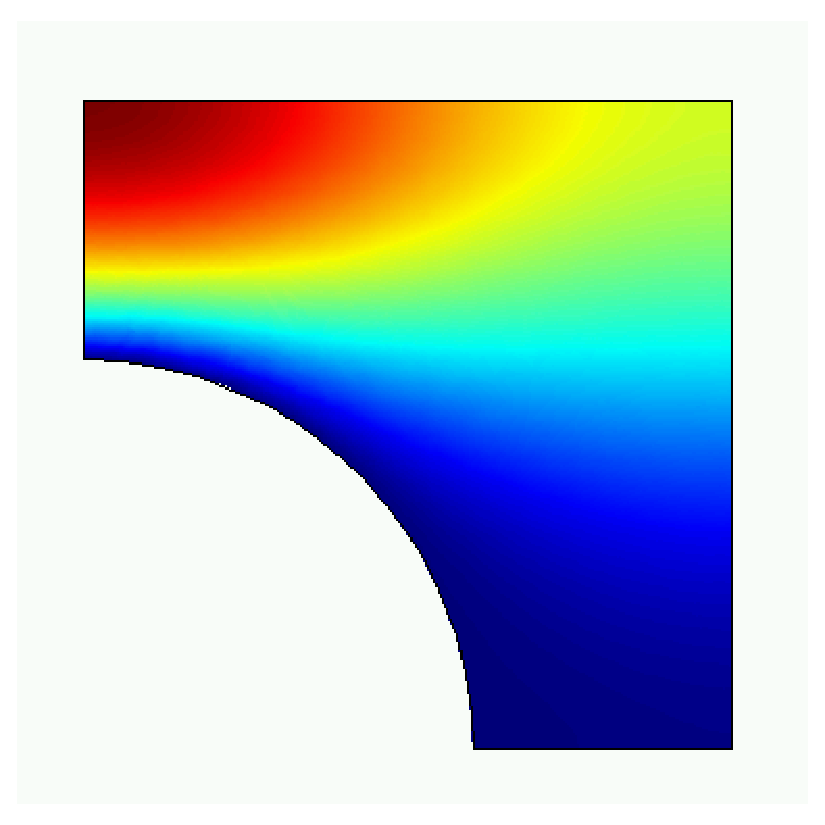
\includegraphics[height=3.5cm]{ns-2d-u.eps}
	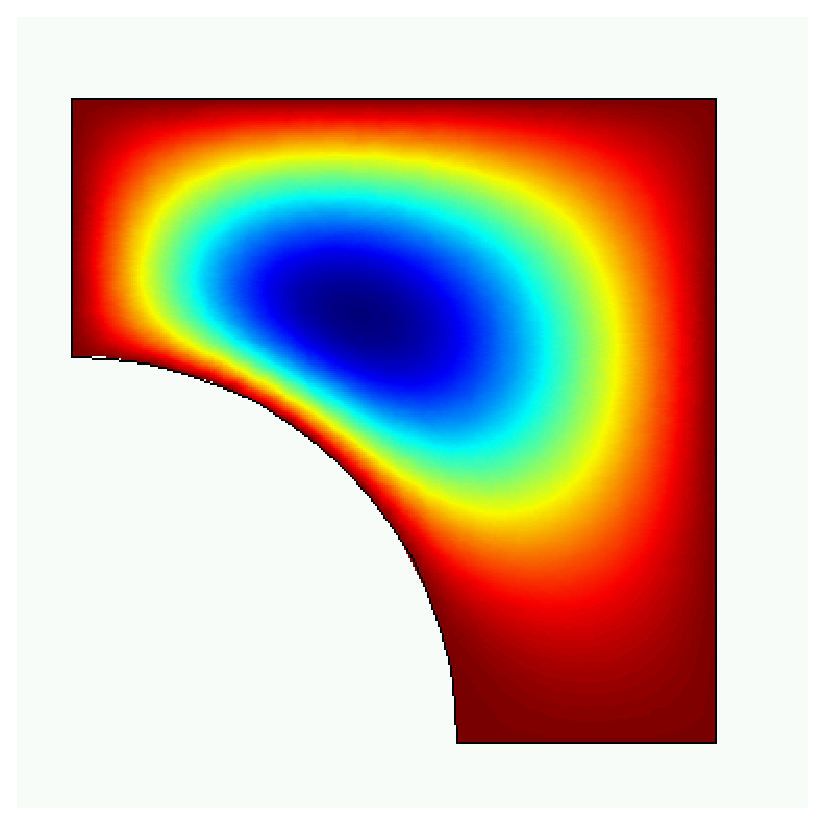
\includegraphics[height=3.5cm]{ns-2d-v.eps}
	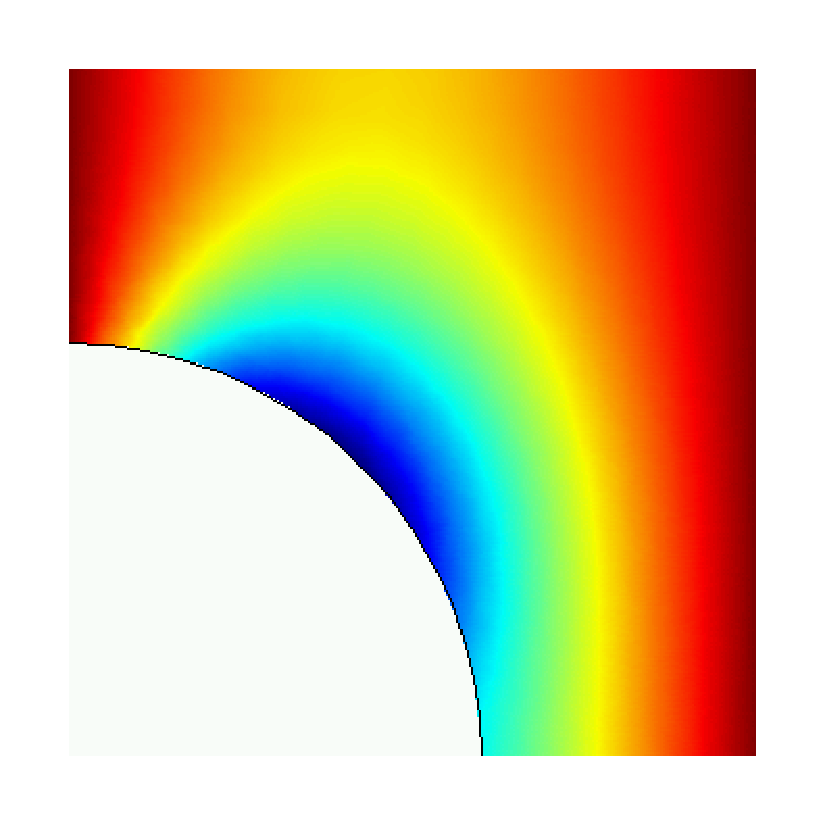
\includegraphics[height=3.4cm]{ns-2d-p.eps}
\end{center}

\begin{center}
	$v_1(x_1,x_2)$ 
	\hspace{2.5cm}
	$v_2(x_1,x_2)$ 
	\hspace{2.5cm}
	$p(x_1,x_2)$ 
\end{center}

\end{slide}

%-------------------------------------------------------------------- Slide --

\overlays{10}{
\begin{slide}{Future plans}

\bigskip

\begin{itemstep}
\item
	Integrate solution to obtain the permeability matrix $K$ in 2D
\item
	Study symmetries of $K$.  Isotropic?

	Heat equation: yes,  Linear elasticity: no
\item
	Extend symmetry calculations to 3D
\item
	Integrate solution to obtain the permeability matrix $K$ in 3D
\item
	Study symmetries of $K$.  Isotropic?
\item
	Investigate the accuracy of solutions as cavity becomes larger

	Limiting case when spheres touch?
\item
	Compute force exerted by one sphere on another
\item
	Compute elastic deformation of a sphere under contact force
\item
	Effect of deformation of spheres on permeability
\end{itemstep}

\fromSlide{10}{\centerline{\red\LARGE THE END}}

\end{slide}
} % end overlays 

%-------------------------------------------------------------------- Slide --

\end{document}
